
\documentclass{beamer}
\usepackage{HECbeamer}
\usepackage{icomma}
\usepackage{numprint}
\title[\color{white}{MATH 60604 \S~6a - Inclusion d'effets de groupe dans la moyenne}]{\texorpdfstring{MATH 60604 \\Modélisation statistique \\ \S~6a - Inclusion d'effets de groupe dans la moyenne}{MATH 60604 \\Modélisation statistique \\ \S~6a - Inclusion d'effets de groupe dans la moyenne}}
\author{}
\institute{HEC Montréal\\
Département de sciences de la décision}
\date{} 

\begin{document}
\frame{\titlepage}

\begin{frame}
 \frametitle{Inclusion d'effets de groupe}
 \bi 
 \item Jusqu'à maintenant, nous avons seulement utilisé la structure de groupe dans la modélisation de la corrélation intra-groupe.
 \item On pourrait également inclure un \alert{effet de groupe} dans la moyenne, ce qui revient à fixer une ordonnée à l'origine différente pour chaque groupe.
 \item Pour ce faire, on ajoute une variable catégorielle \texttt{g} dans le modèle linéaire, ce qui se traduit par l'ajout de $m-1$ indicatrices $\I{\code{g}=i}$ pour $i=1, \ldots, m-1$ s'il y a $m$ groupes. 
 \ei 
 \end{frame}
 \begin{frame}
 \frametitle{Équation avec effets de groupe}
 \bi
 \item Si on inclut dans le modèle les indicatrices pour les niveaux de \code{g}, alors
 \[ Y_{ij}= \beta_0 + \sum_{i=1}^{m-1} \beta_i\I{\code{g}=i} + \eps_{ij},\]
 \bi \item l'ordonnée à l'origine de la catégorie de référence (groupe $m$) est $\beta_0$,
 \item l'effet de groupe pour $\code{g}=i$ est $\beta_i$ $(i=1, \ldots, m-1)$, et 
 \item « l'ordonnée à l'origine spécifique au groupe $i$ » est $\beta_0+ \beta_i$.
 \ei
 \ei
  \end{frame}

\begin{frame}
\frametitle{Modèle linéaire avec effet de groupe - données \texttt{vengeance}}
On considère une régression linéaire ordinaire pour \texttt{vengeance} avec un effet de groupe pour illustrer quelques subtilités.
\bi
\item On désire inclure le fait que le désir de vengeance varie par individu.
\item Nous avons seulement cinq observations par personne pour estimer l'effet groupe.
\item Notre modèle ne prend pas en compte la corrélation intra-individu pour le moment.
\ei
\end{frame}





\begin{frame}[fragile]
\frametitle{Modèle avec effet groupe par individu}
\begin{tcolorbox}[colback=white, colframe=hecblue, title=Code \SASlang pour ajuster un modèle linéaire avec REML]
\begin{verbatim}
proc mixed data=vengeance method=reml; 
class id; 
model vengeance = id sexe age vc wom t / solution; 
run;
\end{verbatim}
\end{tcolorbox}
{\footnotesize En plus de la variable catégorielle \code{id}, le modèle comprend les même variables explicatives qu'avant. Chaque personne a sa propre « ordonnée à l'origine », avec \texttt{id=80} comme catégorie de référence. 


}
\end{frame}

 \begin{frame}
\frametitle{Estimés des paramètres de la moyenne}
\begin{center}
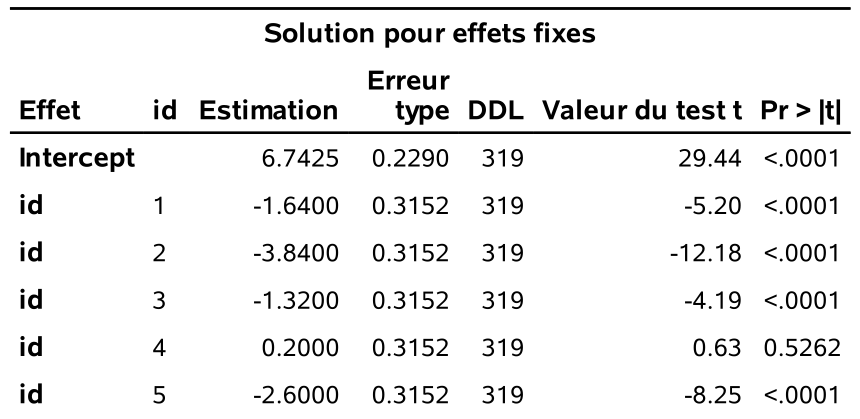
\includegraphics[width = 0.6\linewidth]{img/c6/diapos7-e01}
\begin{align*}
\vdots      
\end{align*}

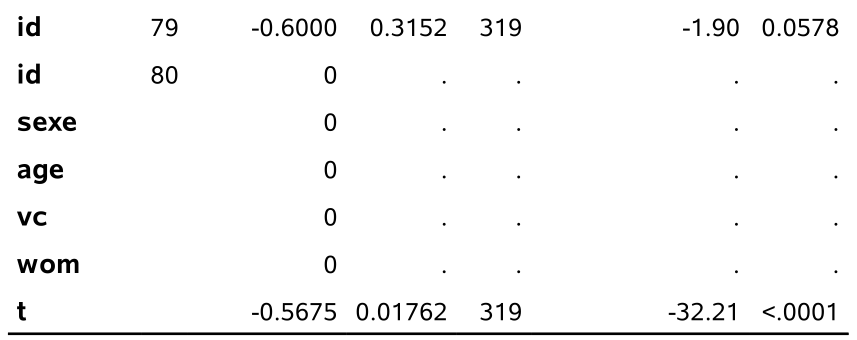
\includegraphics[width = 0.6\linewidth]{img/c6/diapos7-e02}
\end{center}

\end{frame}


 \begin{frame}
\frametitle{Tableau des tests-$F$}
\begin{center}
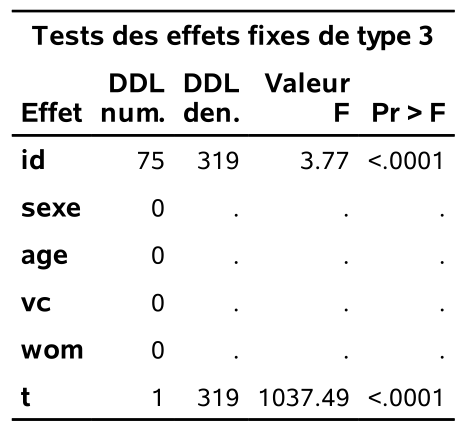
\includegraphics[width=0.4\linewidth]{img/c6/diapos7-e03}
\end{center}
{\footnotesize 

Il n'y \textbf{aucun} paramètre estimé ou test d'hypothèse pour les variables \code{sexe}, \code{age}, \code{vc} or \code{wom}, mais ces derniers sont disponibles pour la variable \code{t}. 
Parce que certaines covariables ne varient pas dans le temps, leur effet n'est pas identifiable (collinéarité parfaite). En retirant \code{id} du modèle, leur effet devient estimable (on obtient $75$ \code{ddl} plutôt que $79$ dans le tableau de tests-$F$).

}
\end{frame}

\begin{frame}[fragile]
\frametitle{Collinéarité}
\bi
\item  En fait, une fois qu'on incorpore un effet individuel pour chaque personne, \alert{il n'est pas possible d'incorporer en même temps une variable explicative qui est fixe dans le temps pour une personne}. 
\item Ici, les variables \code{sexe}, \code{age}, \code{vc} et \code{wom} sont fixes dans le temps pour chaque personne (\code{vc} et \code{wom} ont été mesurées uniquement dans le premier questionnaire).  
\item Ces variables sont donc déjà implicitement incorporées dans l'effet individuel. Techniquement, il y a ici \alert{colinéarité parfaite} entre une variable fixe dans le temps et la variable catégorielle \code{id}. 
\item On peut donc prédire parfaitement la valeur de \code{sexe} uniquement à partir de \code{id} (idem pour les autres covariables fixes). 
\item Ainsi, on ne peut pas avoir simultanément un effet fixe pour chaque personne et incorporer des variables explicatives qui sont fixes pour les personnes.
\ei
\end{frame}

 \begin{frame}
 \frametitle{Défis découlant de l'inclusion d'un effet groupe}
 
 \bi 
 \item La variable groupe est catégorielle: s'il y a peu d'observations par groupe, on ne peut estimer de façon fiable les estimés des coefficients de l'effet groupe.
 \item Si le nombre de groupes $m$ est grand par rapport à la taille totale de l'échantillon, il peut aussi y avoir trop de paramètres dans le modèle. 
 \item On ne peut pas estimer l'effet de variables qui sont fixées au sein des groupes si un effet groupe est inclus.
 \ei
\end{frame}


\begin{frame}[fragile]
\frametitle{Modèle avec effet de groupe et erreurs corrélées}
Le modèle qu'on ajuste inclut seulement \code{id} et la vague du questionnaire \texttt{t} comme variables explicatives pour la moyenne, mais on inclut une structure autorégressive d'ordre un pour la corrélation intra-individu des erreurs $\bs{\eps}$.

\begin{tcolorbox}[colback=white, colframe=hecblue, title=Code \SASlang pour un modèle avec effet groupe et corrélation $\mathsf{AR}(1)$]
\begin{verbatim}
proc mixed data=vengeance method=reml; 
class id tcat; 
model vengeance = id t / solution; 
repeated tcat / subject=id type=ar(1); 
run;
\end{verbatim}
\end{tcolorbox}
{\footnotesize Le paramètre de corrélation du modèle $\mathsf{AR}(1)$ est significativement non-nul (statistique du rapport de vraisemblance de $21,68$ de loi nulle  $\chi^2_1$, valeur-$p$ négligeable). L'estimé de \texttt{t} est $-0,568$, presque le même que dans le modèle incluant \code{sexe}, \code{age}, \code{vc} et \code{wom} avec une structure  $\mathsf{AR}(1)$ du chapitre précédent. 

}
\end{frame}

\begin{frame}[fragile]
\frametitle{Remarque sur la comparaison de modèles}
\bi
\item Il faut faire attention à \alert{ne pas comparer} les critères d'information du modèle avec \code{id} de ceux du modèle avec \code{sexe}, \code{age}, \code{vc} et \code{wom}, car nous avons utilisé la méthode d'estimation REML (option par défaut). 
\item Nous avons mentionné à la section précédente que le $\mathsf{AIC}$ et le $\mathsf{BIC}$ obtenus de la méthode REML, ne sont \textbf{pas comparables} si les variables explicatives de la moyenne (effets fixes) des modèles ne sont pas les mêmes. 
\item Si on veux comparer ces deux modèles, il faut plutôt utiliser la méthode d'estimation du maximum de vraisemblance \texttt{method=ml} dans l'appel à \texttt{proc mixed}.
\ei
 \begin{center}
  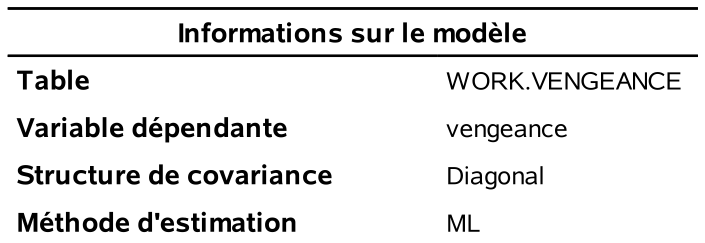
\includegraphics[width = 0.5\linewidth]{img/c6/diapos7-e05}
 \end{center}
   
\end{frame}


\begin{frame}[fragile]
\frametitle{Remarque sur la comparaison de modèles}
On ajuste les deux modèles par maximum de vraisemblance
avec des erreurs autocorrélées (modèle $\mathsf{AR}(1)$).
\begin{center}
\begin{tabular}{c c c r}
\toprule 
\textbf{Modèle} & \textbf{AIC} & \textbf{BIC} & $\hat{\rho}$ (valeur-$p$)\\ \midrule 
\code{sexe}, \code{age}, \code{vc}, \code{wom}, \code{t} & 666,1 & \alert{685,1}  & $0,48$ ($10^{-20}$) \\
\code{id}, \code{t} & \alert{653,4} & 851,1 & $-0,013$ ($0,83$)\\ \bottomrule
\end{tabular}
\end{center}
\bi
\item Le modèle préférable selon le $\mathsf{AIC}$ inclut \code{id}, mais le $\mathsf{AIC}$ tend à choisir des modèles plus compliqués.
\item Le modèle préférable selon le $\mathsf{BIC}$ n'inclut pas l'effet de groupe, mais plutôt \code{sexe}, \code{age}, \code{vc} et \code{wom}.
\item Si on inclut un effet groupe, la corrélation entre les erreurs semble superflue --- l'estimé du coefficient de corrélation est même négatif, ce qui est contre-intuitif et suggère un modèle surparamétrisé.
\ei
\end{frame}

\begin{frame}
\frametitle{Remarque sur la comparaison de modèles}
\bi
\item Le choix des covariables dépend des buts de l'étude. Si on est intéressé par les effets de certaines des variables \code{sexe}, \code{age}, \code{vc} et \code{wom}, alors n'a pas le choix: on choisit le modèle qui les inclut. 
\item Si c'est seulement l'effet du temps qui est d'intérêt, alors les deux modèles mènent à la même conclusion de toute façon.
\item Souvent, l'optimisation échoue --- ça devient difficile d'estimer des paramètres de covariance et un effet fixe de groupe
\item Nous verrons plus loin qu'il est possible d'incorporer à la fois des variables fixes au niveau des groupes (des personnes dans notre exemple) et des effets groupes (\code{id} dans notre exemple) en utilisant des \alert{effets aléatoires}.
\ei
\end{frame}
\end{document}
